\chapter{Implementation}
\label{chap:implementation}

\section{Front end}

\section{Back end}

\subsection{GHC integration}

The front end enables the user to construct Haskell expressions in a convenient manner.
The visual representation is converted into a tree of expression (\code{Expr}) objects and passed to the back end. \index{Expr}
The back end, finally, integrates with the Glasgow Haskell Compiler (\gls{GHC}) to do the actual computation.

The GHC integration is very simplistic.
The back end launches an instance of GHCi, the interactive read-eval-print-loop. \index{REPL}
This \gls{REPL} is then drip-fed the expressions over its standard input stream, converted from the intermediate representation into actual Haskell program code.
If the expression compiles and executes without problems, the result is returned to the front end.

\subsection{Expression and type representation}

\begin{figure}[h]
	\centering
	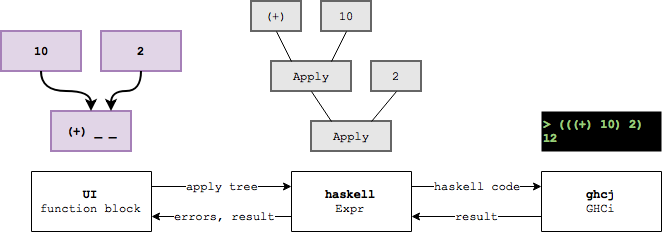
\includegraphics[scale=0.5]{Images/exprtohaskell}
	\label{fig:classdiagram-expr}
	\caption{Translation from visual representation to Haskell code}
\end{figure}

\subsubsection{Expressions}
\index{function} \index{Haskell code}

To be able to work with Haskell code in Java, we built our own representation for the Haskell programming language.
We have chosen to use distinct classes (with a common superclass) for expressions that behave in a similar manner.
This object-based approach is favoured over any text based approach (including using Haskell code itself) because objects are very easy to work with.

Every expression is represented as an instance of \code{Expr} (or any subclass of \code{Expr}). \index{Expr}
An \code{Expr} is responsible for outputting syntactically correct Haskell code. \code{Expr} objects are the bridge between the tree-like graphical representation of the user interface and the textual Haskell code.
The implemented types of expressions are standard functions, values and function applications.
Each of these types of expressions share the fact that they all have a type which can be used by the type checker.

Standard functions (functions that are known to the Haskell environment) are represented as an \code{Ident} instance. \index{Ident}
This class is very simple and does not include more than the name of the function (so it can be called) and a way to lookup the type.

Values are represented in a similar way, a \code{Value} object keeps track of the string representation of the value and its type. \index{Value}
The string representation of the value should be written in a way that GHCi natively understands what is meant by it, altough this is not validated.

Function application is done by using an \code{Apply} object. \index{Apply}
This class holds two expressions where the second expression is applied to the first expression.
\code{Apply} is limited to the application for a single argument.
A function with more than one argument is seen as a function with one argument that produces another function.
This way \code{Apply} allows for creating a tree like structure of a Haskell program.

Custom functions can be built using a composition of standard functions.
A custom function is defined using a \code{Function} object.
This object requires a specification of the function arguments and the expression tree of the function.
A \code{FunctionArgument} object can be used in this expression tree to use the inputs.
Functions that are defined this way will make sure that type calculations are done on a per-usage basis so reusing a function is always possible.
When a function is pushed to GHCi an \code{Ident} object is given which can be used instead of the \code{Function} object.
This comes with a great performance gain because the function itself is not continuously type checked.

Once a program has been represented as a tree of \code{Expr} objects, calling the \code{Expr.analyze()} method will invoke the type checker.
The type checker calculates the new types for the expressions in the tree.
The new types of each expression can be obtained by calling the \code{Expr.getType()} method.
This way it is possible to always get the up-to-date type of an \code{Expr} object by simply keeping a reference to it.

\begin{figure}[h]
\centering
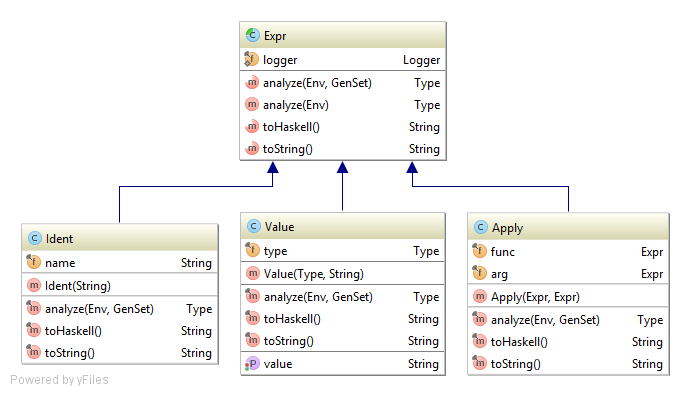
\includegraphics[scale=0.4]{Images/classdiagram-expr}
\label{fig:classdiagram-expr}
\caption{Class diagram of the Haskell expressions classes}
\end{figure}

\subsubsection{Types}
\index{type}

Types are represented similarly to expressions.
Each type is represented as an instance of \code{Type} (or any subclass of it).
The subclasses of \code{Type} are used to make working with types easier.
There is no subclass for every distinct type in Haskell, only for groups of types that are alike.

First of all types are separated into two groups: variable types and nonvariable types.
Variable types are types of which the actual type is not known - types that can unify into any nonvariable type (possibly with constraints).
Variable types are represented as \code{VarT}.

Nonvariable types (constant types) are represented as \code{ConstT} and consist of a type constructor and a number of (optional) argument types.
A type is considered constant when it is clear which type constructor to use. A type with a known type constructor but variable types as argument types is still a constant type.

Composite types, e.g. list and tuple, are represented by respectively \code{ListT} and \code{TupleT} which are subclasses of \code{ConstT}.
These subclasses handle some validation and Haskell/string representation that is specific to these types.

Distinct Haskell types are represented as class instances, not as the class itself. The different \code{Type} subclasses make it easier to work with the types, and some are necessary in case of compound types like \code{ListT} and \code{TupleT} which are special cases.

Non-variable types can be easily compared. Two instances of the same type are equal (that is, two instances with the same base class and constructor arguments).
Variable types are only equal if it is the same instance. This is used to avoid confusion between variable types with the same name.

Type classes are represented as \code{TypeClass} instances and can be used as constraints on variable types.
Each \code{TypeClass} instance keeps a set of constant types that belong to the type class.
This information is used by the type checker to check whether a variable type is unifyable with a constant type or another variable type.

\begin{figure}[h]
\centering
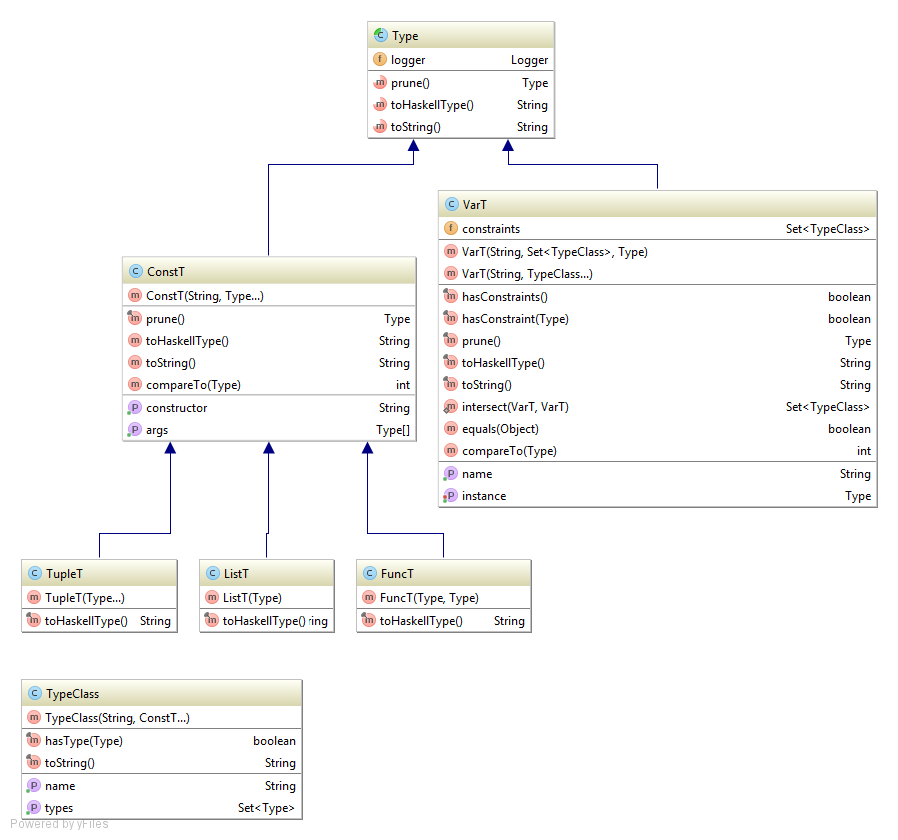
\includegraphics[scale=0.4]{Images/classdiagram-type}
\label{fig:classdiagram-type}
\caption{Class diagram of the Haskell types classes}
\end{figure}

\subsection{Type checker}

From our own experience as beginning Haskell programmers, we often encountered type errors, and therefore GHC's type error messages.
Very early in the project, we decided that the back end had to do at least some type-related work itself, to provide better errors to the user, and also to be able to show type hints, without having to parse GHC's error messages.
Not long thereafter, it was decided that such a home-grown type checker would not need to support the entirety of Haskell's type system.

After some iterations, we have arrived at an approach that could probably be described as a subset of Hindley-Milner type inference. \index{Hindley-Milner} \index{type inference}

Our (Java) implementation of Hindley-Milner type inference is based on an implementation in Scala by Andrew Forrest\cite{forrest}.
This implementation was in turn based on an implementation in Perl by Nikita Borisov\cite{borisov}.
The Perl implementation was heavily inspired by a Modula-2 implementation from 1987 by Luca Cardelli\cite{cardelli}.
Some ideas were also taken from the chapter on types from the programming languages book by Krishnamurthi\cite{plai}.

As mentioned, the type checker is not nearly powerful enough to understand or even represent the entire complexity of Haskell's type system.
However, we have found it to be `good enough' for our purposes.

\subsection{Environment management}

In Haskell a lot of things depend on the environment, for example the functions that are available, the types in type classes, etc.
Our implementation solves this by introducing an environmet (\code{Env}).
Objects of this class keep the types of the available functions and the type classes for every type.
Furthermore, we provide a XML-based catalog where the initial functions and type classes can be configured.
This catalog contains information that can be used by the front end, such as documentation as well.